\thispagestyle{plain}
\section{Recta Num\'erica, Densidad y Orden}
La recta numérica es una línea recta en la que se representan los números reales. La recta numérica es una forma de representar los números reales en una línea recta. En ella, cada punto representa un número real. Los números se pueden representar y se pueden comparar los números reales en la recta numérica.

\subsection{Orden de fracciones y decimales}

\subsubsection{Orden en los n\'umeros fraccionarios}
Para comparar fracciones, debemos convertirlas a un mismo denominador. Por ejemplo, para comparar $\frac{1}{2}$ y $\frac{3}{4}$, debemos convertirlas a un mismo denominador. El mínimo común múltiplo de $2$ y $4$ es $4$, por lo que debemos convertir $\frac{1}{2}$ a $\frac{2}{4}$, y $\frac{3}{4}$ a $\frac{3}{4}$. Ahora podemos compararlas, y vemos que:

\[\frac{2}{4}<\frac{3}{4}\]

\begin{center}
    \begin{tikzpicture}[scale=1]
        % Recta numérica
        \draw[latex-latex] (-0.8,0) -- (10.2,0);

        % Números racionales entre 0 y 1
        \foreach \x in {0,2.5,5,7.5,10}
        \draw (\x,0.1) -- (\x,-0.1);

        % Etiquetas de números racionales
        \foreach \x/\label in { 0/{0}, 2.5/{\dfrac{1}{4}}, 5/{{\color{gray}\dfrac{1}{2}=}\dfrac{2}{4}}, 7.5/{\dfrac{3}{4}},10/{1}}
        \node[below] at (\x,-0.1) {$\label$};

        % Puntos rojo y verde
        \fill[color=red!50!black] (5,0) circle (0.16);
        \fill[color=red!50!black] (7.5,0) circle (0.16);
    \end{tikzpicture}
\end{center}

\subsubsection{Orden en los n\'umeros decimales}

Para comparar decimales, debemos convertirlos a un mismo número de decimales. Por ejemplo, para comparar $0.5$ y $0.35$, debemos convertirlos a un mismo número de decimales. El número de decimales de $0.5$ es $1$, y el número de decimales de $0.35$ es $2$. Para convertir $0.5$ a $0.50$, debemos agregar un $0$ al final. Ahora podemos compararlos, y vemos que:

\[0.50>0.35\]

\begin{center}
    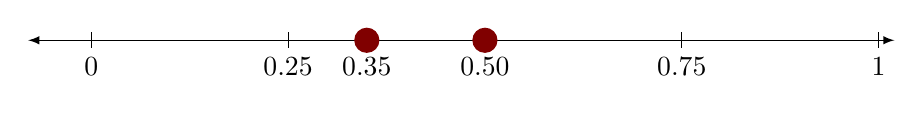
\begin{tikzpicture}[scale=1]
        % Recta numérica
        \draw[latex-latex] (-0.8,0) -- (10.2,0);

        % Números racionales entre 0 y 1
        \foreach \x in {0,2.5,5,7.5,10}
        \draw (\x,0.1) -- (\x,-0.1);

        % Etiquetas de números racionales
        \foreach \x/\label in { 0/{0}, 2.5/{0.25}, 3.5/{0.35}, 5/{0.50}, 7.5/{0.75},10/{1}}
        \node[below] at (\x,-0.1) {$\label$};

        % Puntos rojo y verde
        \fill[color=red!50!black] (5,0) circle (0.16);
        \fill[color=red!50!black] (3.5,0) circle (0.16);
    \end{tikzpicture}
\end{center}

\subsection{Densidad de fracciones y decimales}

En teoría de conjuntos, se dice que un conjunto numérico es \textbf{denso}, si entre dos elementos cualesquiera del conjunto, existe otro elemento del conjunto. Por ejemplo, el conjunto de los números racionales es denso, porque entre dos números racionales cualesquiera, existe otro número racional.

Por ejemplo, entre $\frac{1}{2}$ y $\frac{3}{4}$, existe $\frac{5}{8}$.\\

% Representacion detallada en Tikz de una recta numérica que muestra la densidad de los números racionales. 
% Se muestra la recta numérica con los números racionales entre 0 y 1, y se muestra con etiquetas que entre dos números racionales como el 1/2 y  el 3/4,
% existe otro número racional como el 5/8.
\begin{tikzpicture}[scale=2]
    % Recta numérica
    \draw[latex-latex] (4,0) -- (8,0);

    % Números racionales entre 0 y 1
    \foreach \x in { 5, 6, 7  }
    \draw (\x,0.1) -- (\x,-0.1);

    % Etiquetas de números racionales
    \foreach \x/\label in { 5/{\dfrac{1}{2}}, 6.25/{\dfrac{5}{8}}, 7.5/{\dfrac{3}{4}}}
    \node[below] at (\x,-0.1) {$\label$};

    % Puntos rojo y verde
    \fill[color=red!50!black] (5,0) circle (0.08);
    \fill[color=red!50!black] (7.5,0) circle (0.08);
    \fill[color=green!50!black] (6.25,0) circle (0.08);
\end{tikzpicture}

Si observamos ahora en medio del $\frac{1}{2}$ y el $\frac{5}{8}$, está el $\frac{9}{16}$.\\

% Representacion detallada en Tikz de una recta numérica que muestra la densidad de los números racionales. 
% Se muestra la recta numérica con los números racionales entre 0 y 1, y se muestra con etiquetas que entre dos números racionales como el 1/2 y  el 5/8,
% existe otro número racional como el 9/16
\begin{tikzpicture}[scale=2]
    % Recta numérica
    \draw[latex-latex] (4,0) -- (8,0);

    % Números racionales entre 0 y 1
    \foreach \x in {  5, 6, 7}
    \draw (\x,0.1) -- (\x,-0.1);

    % Etiquetas de números racionales
    \foreach \x/\label in {5/{\dfrac{1}{2}}, 5.625/{\dfrac{9}{16}}, 6.25/{\dfrac{5}{8}}, 7.5/{\dfrac{3}{4}}}
    \node[below] at (\x,-0.1) {$\label$};

    % Puntos rojo y verde
    \fill[color=red!50!black] (5,0) circle (0.08);
    \fill[color=green!50!black] (6.25,0) circle (0.08);
    \fill[color=red!50!black] (7.5,0) circle (0.08);
    \fill[color=blue!50!black] (5.625,0) circle (0.08);
\end{tikzpicture}

Y si observamos ahora en medio del $\frac{1}{2}$ y el $\frac{9}{16}$, esta el $\frac{19}{32}$.\\

% Representacion detallada en Tikz de una recta numérica que muestra la densidad de los números racionales.
% Se muestra la recta numérica con los números racionales entre 0 y 1, y se muestra con etiquetas que entre dos números racionales como el 1/2 y  el 9/16,
% existe otro número racional como el 19/32

\begin{tikzpicture}[scale=2]
    % Recta numérica
    \draw[latex-latex] (4,0) -- (8,0);

    % Números racionales entre 0 y 1
    \foreach \x in {  5, 6, 7}
    \draw (\x,0.1) -- (\x,-0.1);

    % Etiquetas de números racionales
    \foreach \x/\label in {5/{\dfrac{1}{2}}, 5.3125/{\dfrac{19}{32}}, 5.625/{\dfrac{9}{16}}, 6.25/{\dfrac{5}{8}}, 7.5/{\dfrac{3}{4}}}
    \node[below] at (\x,-0.1) {$\label$};
    % Puntos rojo y verde
    \fill[color=red!50!black] (5,0) circle (0.08);
    \fill[color=green!50!black] (6.25,0) circle (0.08);
    \fill[color=red!50!black] (7.5,0) circle (0.08);
    \fill[color=blue!50!black] (5.625,0) circle (0.08);
    \fill[color=yellow!50!black] (5.3125,0) circle (0.08);
\end{tikzpicture}

\subsubsection{Densidad de los decimales}
Los decimales también son densos. Por ejemplo, entre $0.5$ y $0.6$, existe $0.55$.\\

% Representacion detallada en Tikz de una recta numérica que muestra la densidad de los números decimales.
% Se muestra la recta numérica con los números decimales entre 0 y 1, y se muestra con etiquetas que entre dos números decimales como el 0.5 y  el 0.6,
% existe otro número decimal como el 0.55
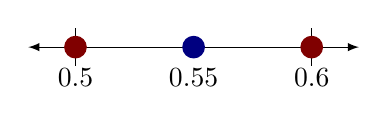
\begin{tikzpicture}[scale=3]
    % Recta numérica
    \draw[latex-latex] (4.8,0) -- (6.2,0);

    % Números decimales entre 0 y 1
    \foreach \x in {  5, 6}
    \draw (\x,0.08) -- (\x,-0.08);

    % Etiquetas de números decimales
    \foreach \x/\label in {5/{0.5}, 5.5/{0.55}, 6/{0.6}}
    \node[below] at (\x,-0.05) {$\label$};

    % Puntos rojo y verde
    \fill[color=red!50!black] (5,0) circle (0.048);
    \fill[color=red!50!black] (6,0) circle (0.048);
    \fill[color=blue!50!black] (5.5,0) circle (0.048);
\end{tikzpicture}

Si observamos de cerca ahora en medio del $0.5$ y el $0.55$, esta el $0.525$.\\

% Representacion detallada en Tikz de una recta numérica que muestra la densidad de los números decimales.
% Se muestra la recta numérica con los números decimales entre 0 y 1, y se muestra con etiquetas que entre dos números decimales como el 0.5 y  el 0.55,
% existe otro número decimal como el 0.525
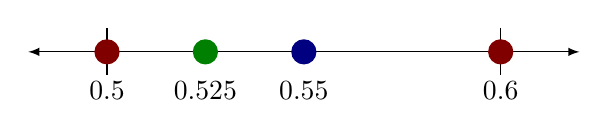
\begin{tikzpicture}[scale=5]
    % Recta numérica
    \draw[latex-latex] (4.8,0) -- (6.2,0);
    % Números decimales entre 0 y 1
    \foreach \x in {  5, 6}
    \draw (\x,0.06) -- (\x,-0.06);
    % Etiquetas de números decimales
    \foreach \x/\label in {5/{0.5}, 5.25/{0.525}, 5.5/{0.55}, 6/{0.6}}
    \node[below] at (\x,-0.05) {$\label$};
    % Puntos rojo y verde
    \fill[color=red!50!black] (5,0) circle (0.032);
    \fill[color=red!50!black] (6,0) circle (0.032);
    \fill[color=blue!50!black] (5.5,0) circle (0.032);
    \fill[color=green!50!black] (5.25,0) circle (0.032);
\end{tikzpicture}

Y si observamos de cerca ahora en medio del $0.5$ y el $0.525$, esta el $0.5125$.\\

% Representacion detallada en Tikz de una recta numérica que muestra la densidad de los números decimales.
% Se muestra la recta numérica con los números decimales entre 0 y 1, y se muestra con etiquetas que entre dos números decimales como el 0.5 y  el 0.525,
% existe otro número decimal como el 0.5125
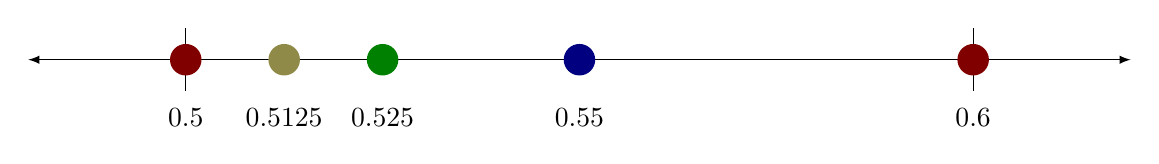
\begin{tikzpicture}[scale=10]
    % Recta numérica
    \draw[latex-latex] (4.8,0) -- (6.2,0);
    % Números decimales entre 0 y 1
    \foreach \x in {  5, 6}
    \draw (\x,0.04) -- (\x,-0.04);
    % Etiquetas de números decimales
    \foreach \x/\label in {5/{0.5}, 5.125/{0.5125}, 5.25/{0.525}, 5.5/{0.55}, 6/{0.6}}
    \node[below] at (\x,-0.05) {$\label$};
    % Puntos rojo y verde
    \fill[color=red!50!black] (5,0) circle (0.02);
    \fill[color=red!50!black] (6,0) circle (0.02);
    \fill[color=blue!50!black] (5.5,0) circle (0.02);
    \fill[color=green!50!black] (5.25,0) circle (0.02);
    \fill[color=yellow!50!black] (5.125,0) circle (0.02);
\end{tikzpicture}

A esta propiedad de los números racionales (fracciones, decimales y enteros), se le llama \textbf{densidad}.
\newpage